\documentclass[a4paper, article, oneside, USenglish, hidelinks]{memoir}

%% Encoding
\usepackage[utf8]{inputenc}
\usepackage[T1]{fontenc}


%% Color
\usepackage{xcolor}


%% Fonts and typography
\usepackage{lmodern}           % Latin Modern Roman
\usepackage[scaled]{beramono}  % Bera Mono (Bitstream Vera Sans Mono)
\renewcommand{\sfdefault}{phv} % Helvetica
\usepackage[final]{microtype}  % Improved typography
\usepackage{caladea}

\pretitle{\begin{center}\LARGE\sffamily\bfseries}                    % Title
\renewcommand{\abstractnamefont}{\sffamily\bfseries}                 % Abstract
\renewcommand*{\chaptitlefont}{\LARGE\bfseries\sffamily\raggedright} % Chapter
\setsecheadstyle{\Large\bfseries\sffamily\raggedright}               % Section
\setsubsecheadstyle{\large\bfseries\sffamily\raggedright}               % Section


%% small gap between paragraphs
%\setlength{\parskip}{2pt}


%% Mathematics
\usepackage{amssymb}   % Extra symbols
\usepackage{mathtools} % Fonts and environments for mathematical formuale


%% Miscellanous
\usepackage{graphicx}  % Tool for images
\usepackage{babel}     % Automatic translations
\usepackage{textcomp}  % Extra symbols
\usepackage{lipsum}

%% Code snippets
\definecolor{source_blue}{HTML}{003399}
\definecolor{source_brown}{HTML}{AAAA53}
\definecolor{source_gray}{HTML}{F9F9F9}
\definecolor{source_orange}{HTML}{E18A07}
\definecolor{dkgreen}{rgb}{0,0.6,0}
\usepackage{listings}  % Typesetting code
\lstset{
	basicstyle=\ttfamily\footnotesize,
	breaklines=true,
	keepspaces=true,
	tabsize=4,
	numbers=left,
	numberstyle=\ttfamily\color{darkgray},
	backgroundcolor=\color{source_gray},
	rulecolor=\color{gray},
	xleftmargin=2.7em,
	frame=single,
	framexleftmargin=2.4em,
	showstringspaces=false,
	language=TeX,
	morekeywords={\documentclass,\begin,\end,\usepackage,\makeinvoice,\setinvoicetitle,\setinvoicenumber,\setreceivername,\setreceiveraddress,\setname,\setaddress,\setphonenumber,\setemail,\setyourref,\setourref,\setinvoicedate,\setdeadline,\additem,\setsubtotal,\setvat,\settotal,\setaccountnumber},
	commentstyle=\color{source_brown}\ttfamily, 
	keywordstyle=\color{source_blue}\ttfamily,
	stringstyle=\color{source_orange},
	literate={æ}{{\ae}}1{ø}{{\o}}1{å}{{\aa}}1
}


%% Cross references
\usepackage{varioref}
\usepackage{hyperref}
\usepackage[nameinlink, capitalize, noabbrev]{cleveref}


% Allow longer words
\tolerance = 5000 
\hbadness = \tolerance 
\pretolerance = 2000 


\usepackage{pdfpages}
%\usepackage{simpleinvoice}


\title{The \texttt{simpleinvoice} Package}
\author{Mathias Lohne}
\date{}


\begin{document}
\maketitle

\tableofcontents

\newpage
\chapter{Package overview}
The \texttt{simpleinvoice} package lets you easily typeset professional-looking invoices, and makes sure that all the legally required information is on the invoice. 

The package respects the global language set in the document, or can be loaded with another language specified. The languages currently supported are English and Norwegian (bokmål).


Following are a list of all available commands, detailed description are available in \cref{sec:commanddetails}.

\begin{itemize}
	\item \nameref{par:setinvoicenumber}
	\item \nameref{par:setreceivername}
	\item \nameref{par:setreceiveraddress}
	\item \nameref{par:setname}
	\item \nameref{par:setaddress}
	\item \nameref{par:setphonenumber}
	\item \nameref{par:setemail}
	\item \nameref{par:setyourref}
	\item \nameref{par:setourref}
	\item \nameref{par:setinvoicedate}
	\item \nameref{par:setdeadline}
	\item \nameref{par:additem}
	\item \nameref{par:setsubtotal}
	\item \nameref{par:setvat}
	\item \nameref{par:settotal}
	\item \nameref{par:setaccountnumber}
	\item \nameref{par:makeinvoice}
\end{itemize}


\newpage
\chapter{Detailed descriptions}

 
\section{Loading package}
The package is loaded with the \verb|\usepackage| command. If no language is specified in the options, the package defaults to the document langugae.
\begin{lstlisting}
\documentclass[english]{article}

\usepackage{simpleinvoice}          % Falls back to english
% OR
\usepackage[norsk]{simpleinvoice}   % Specifies norwegian

\begin{document}

\makeinvoice

\end{document}
\end{lstlisting}


\section{Description of all available commands}
\label{sec:commanddetails}
\subsection{{\textbackslash}setinvoicetitle} 
Overrides the standard title of the invoice. Optional command. Takes one argument: the new title.
Example:
\begin{lstlisting}
\setinvoicetitle{My invoice}
\end{lstlisting}

\subsection{{\textbackslash}setinvoicenumber} \label{par:setinvoicenumber}
Sets the invoice number for the invoice. This command must be present, if not the text ``{\color{red}No number}'' is printed in place of an invoice number. Takes one argument: the invoice number. Example:
\begin{lstlisting}
\setinvoicenumber{42}
\end{lstlisting}

\subsection{{\textbackslash}setreceivername} \label{par:setreceivername}
Sets the receiver name for the invoice. This command must be present, if not the text ``{\color{red}Company name}'' is printed in place of an receiver. Takes one argument: the receiver name. Example:
\begin{lstlisting}
\setreceivername{Person McNameface}
\end{lstlisting}



\subsection{{\textbackslash}setreceiveraddress} \label{par:setreceiveraddress}
Specifies the address for the receiver of the invoice. This command must be present, if not the text ``{\color{red}Address line 1 (newline) Address line 2}'' is printed in place of an address. Takes one argument: a multi-line representation of the address. Example:
\begin{lstlisting}
\setreceiveraddress{Roadname 35C \\ 52353 Cityville}
\end{lstlisting}



\subsection{{\textbackslash}setname} \label{par:setname}
Specifies your (the sender's) name. This command must be present, if not the text ``{\color{red}Your name}'' is printed in place of a name. Takes one argument: your name on a single line.
\begin{lstlisting}
\setname{My Name}
\end{lstlisting}



\subsection{{\textbackslash}setaddress} \label{par:setaddress}
Specifies your (the sender's) address. This command must be present, if not the text ``{\color{red}Address line 1 (newline) Address line 2}'' is printed in place of an address. Takes two arguments: a multi-line representation of the address, and a single-line representation (for the invoice footer).
\begin{lstlisting}
\setaddress{Streetname 4644C \\ 0000 City}{Streetname 4644C / 0000 City}
\end{lstlisting}



\subsection{{\textbackslash}setphonenumber} \label{par:setphonenumber}
Sets your (the sender's) phone number. This command is optional, it is omitted from the invoice if not present. Takes one argument: a telephone number. Example:
\begin{lstlisting}
\setphonenumber{123 45 678}
\end{lstlisting}


\subsection{{\textbackslash}setemail} \label{par:setemail}
Sets your (the sender's) email address. This command is optional, it is omitted from the invoice if not present. Takes one argument: a valid email address. Example:
\begin{lstlisting}
\setemail{mail@domain.com}
\end{lstlisting}

\subsection{{\textbackslash}setyourref} \label{par:setyourref}
Specifies the receiver's reference to the invoice, usually the person in the company you are billing that you have been in contact with. If the invoice is sent to a singe person, that person is their own reference.  This command is optional, it is omitted from the invoice if not present (it is however highly suggested to include this). Takes one argument: a name. Example:
\begin{lstlisting}
\setyourref{Person McNameface}
\end{lstlisting}


\subsection{{\textbackslash}setourref} \label{par:setourref}
Specifies your reference to the invoice (usually your own name, but if the invoice is sent by a company, this could be a specific employee). This command is optional, it is omitted from the invoice if not present (it is however highly suggested to include this). Takes one argument: a name. Example:
\begin{lstlisting}
\setourref{My Name}
\end{lstlisting}



\subsection{{\textbackslash}setinvoicedate} \label{par:setinvoicedate}
Specify the date of the invoice. This command is optional, and the result of \verb|\today| will be written if this command is omitted. Takes one argument: a date. Example:
\begin{lstlisting}
\setinvoicedate{April 1, 2017}
\end{lstlisting}


\subsection{{\textbackslash}setdeadline} \label{par:setdeadline}
Specify the deadline of the invoice. This command is optional, and the deadline is set to 14 days from today if the command is omitted. Takes one argument: number of days later than invoice date. Example:
\begin{lstlisting}
\setdeadline{21}     % extends deadline to April 22, 2017
\end{lstlisting}


\subsection{{\textbackslash}additem} \label{par:additem}
Adds an item to the invoice. At least one instance of this command must be present. Otherwise, ``{\color{red}No items yet}'' is printed. Takes four arguments: item description, item price, VAT percentage, and total price (including VAT). Example:
\begin{lstlisting}
\additem{4 chairs}{100 USD}{0}{400 USD}
\additem{1 table}{250 USD}{0}{250 USD}
\end{lstlisting}


\subsection{{\textbackslash}setsubtotal} \label{par:setsubtotal}
Specify the subtotal of all items before VAT is applied. This command must be present, otherwise ``{\color{red}Subtotal}'' is written in place. Takes one argument: the subtotal. Example:
\begin{lstlisting}
\setsubtotal{650 USD}
\end{lstlisting}


\subsection{{\textbackslash}setvat} \label{par:setvat}
Specify the amount of money given as sales tax for the sale (total). This command must be present, otherwise ``{\color{red}VAT}'' is written in place. Takes one argument: the total VAT. Example:
\begin{lstlisting}
\setvat{0 USD}
\end{lstlisting}


\subsection{{\textbackslash}settotal} \label{par:settotal}
Specify the total of all items after VAT is applied. This command must be present, otherwise ``{\color{red}Total}'' is written in place. Takes one argument: the total. Example:
\begin{lstlisting}
\settotal{650 USD}
\end{lstlisting}


\subsection{{\textbackslash}setaccountnumber} \label{par:setaccountnumber}
Specify the bank account for payment. This command must be present, otherwise ``{\color{red}Bank account}'' is written in place. Takes one argument: the bank account for payment. Example:
\begin{lstlisting}
\setaccountnumber{1234 56 78910}
\end{lstlisting}


\subsection{{\textbackslash}makeinvoice} \label{par:makeinvoice}
Creates the specified invoice. Must be called after all the specifications has been set. Takes no arguments. Example:
\begin{lstlisting}
\makeinvoice
\end{lstlisting}

\chapter{Example invoices}
Following are two different invoices. First, we create the invoice specified in \cref{sec:commanddetails}. The code for this invoice is as follows:
\begin{lstlisting}
\documentclass[english]{article}

\usepackage{simpleinvoice}

\begin{document}

\setinvoicetitle{My Invoice}
\setinvoicenumber{42}

\setreceivername{Person McNameface}
\setreceiveraddress{Roadname 35C \\ 52353 Cityville}

\setname{My Name}
\setaddress{Streetname 4644C \\ 0000 City}{Streetname 4644C / 0000 City}
\setphonenumber{123 45 678}
\setemail{mail@domain.com}

\setyourref{Person McNameface}
\setourref{My Name}

\setinvoicedate{April 1, 2017}
\setdeadline{21}     % extends deadline to April 22, 2017

\additem{4 chairs}{100 USD}{0}{400 USD}
\additem{1 table}{250 USD}{0}{250 USD}

\setsubtotal{650 USD}
\setvat{0 USD}
\settotal{650 USD}
\setaccountnumber{1234 56 78910}
\makeinvoice

\end{document}
\end{lstlisting}
Which yields the result on the next page:\newpage
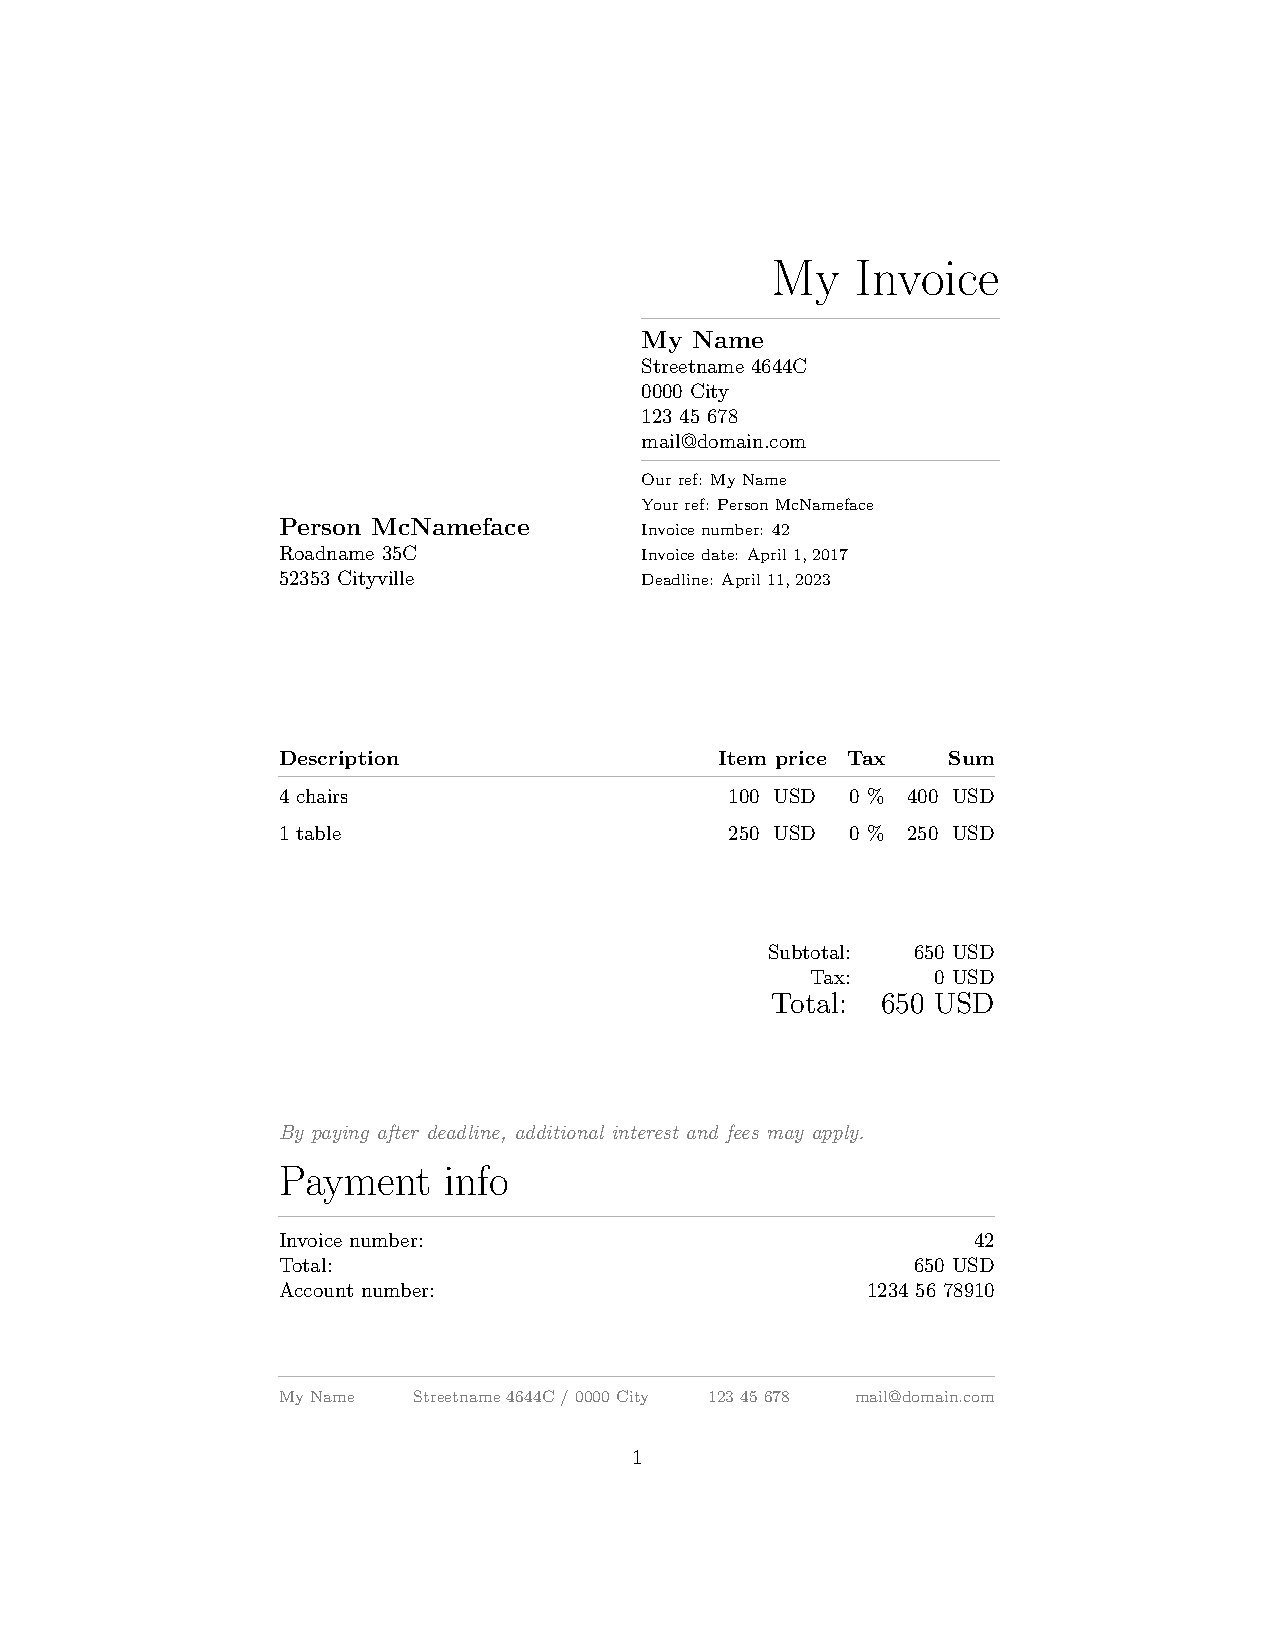
\includepdf{examples/english.pdf}

The \texttt{simpleinvoice} package behaves well with other styling options, such as loading other fonts, and specifying margins. Another example, this time in Norwegian, utilizing more styling options is found below:
\begin{lstlisting}
\documentclass[a4paper, article, oneside, norsk, hidelinks, 10pt]{memoir}

%% Smaller margins
\usepackage[margin=1in]{geometry}

%% Encoding
\usepackage[utf8]{inputenc}
\usepackage[T1]{fontenc}

%% Fonts and typography
\usepackage[final]{microtype}         % Improved typography
\usepackage[sfdefault]{ClearSans}     % Sans serif font

%% Miscellanous styling
\pagestyle{empty}                     % Remove page number

% Invoice
\usepackage{simpleinvoice}

\begin{document}

\setname{Navn Navnesen}
\setaddress{Langtvekkveien 13b \\ 0123 Oslo}{Langtvekkveien 13b / 0123 Oslo}
\setaccountnumber{1234 56 78910}
\setourref{Navn Navnesen}
\setemail{mail@domain.no}
\setphonenumber{123 45 678}

\setreceivername{Rik Rikmansen og sønner}
\setreceiveraddress{Pengeveien 342 \\ 9876 Gokk}
\setyourref{Rik Rikmansen}

\setinvoicenumber{38}

\additem{Flere}{5 000.00 kr}{20}{6 000.00 kr}
\additem{Ulike}{8 000.00 kr}{20}{9 600.00 kr}
\additem{Ting}{10 000.00 kr}{20}{12 000.00 kr}

\setsubtotal{23 000.00 kr}
\setvat{4 600.00 kr}
\settotal{27 600.00 kr}

\makeinvoice

\end{document}
\end{lstlisting}
This yields the result on the next page.\newpage
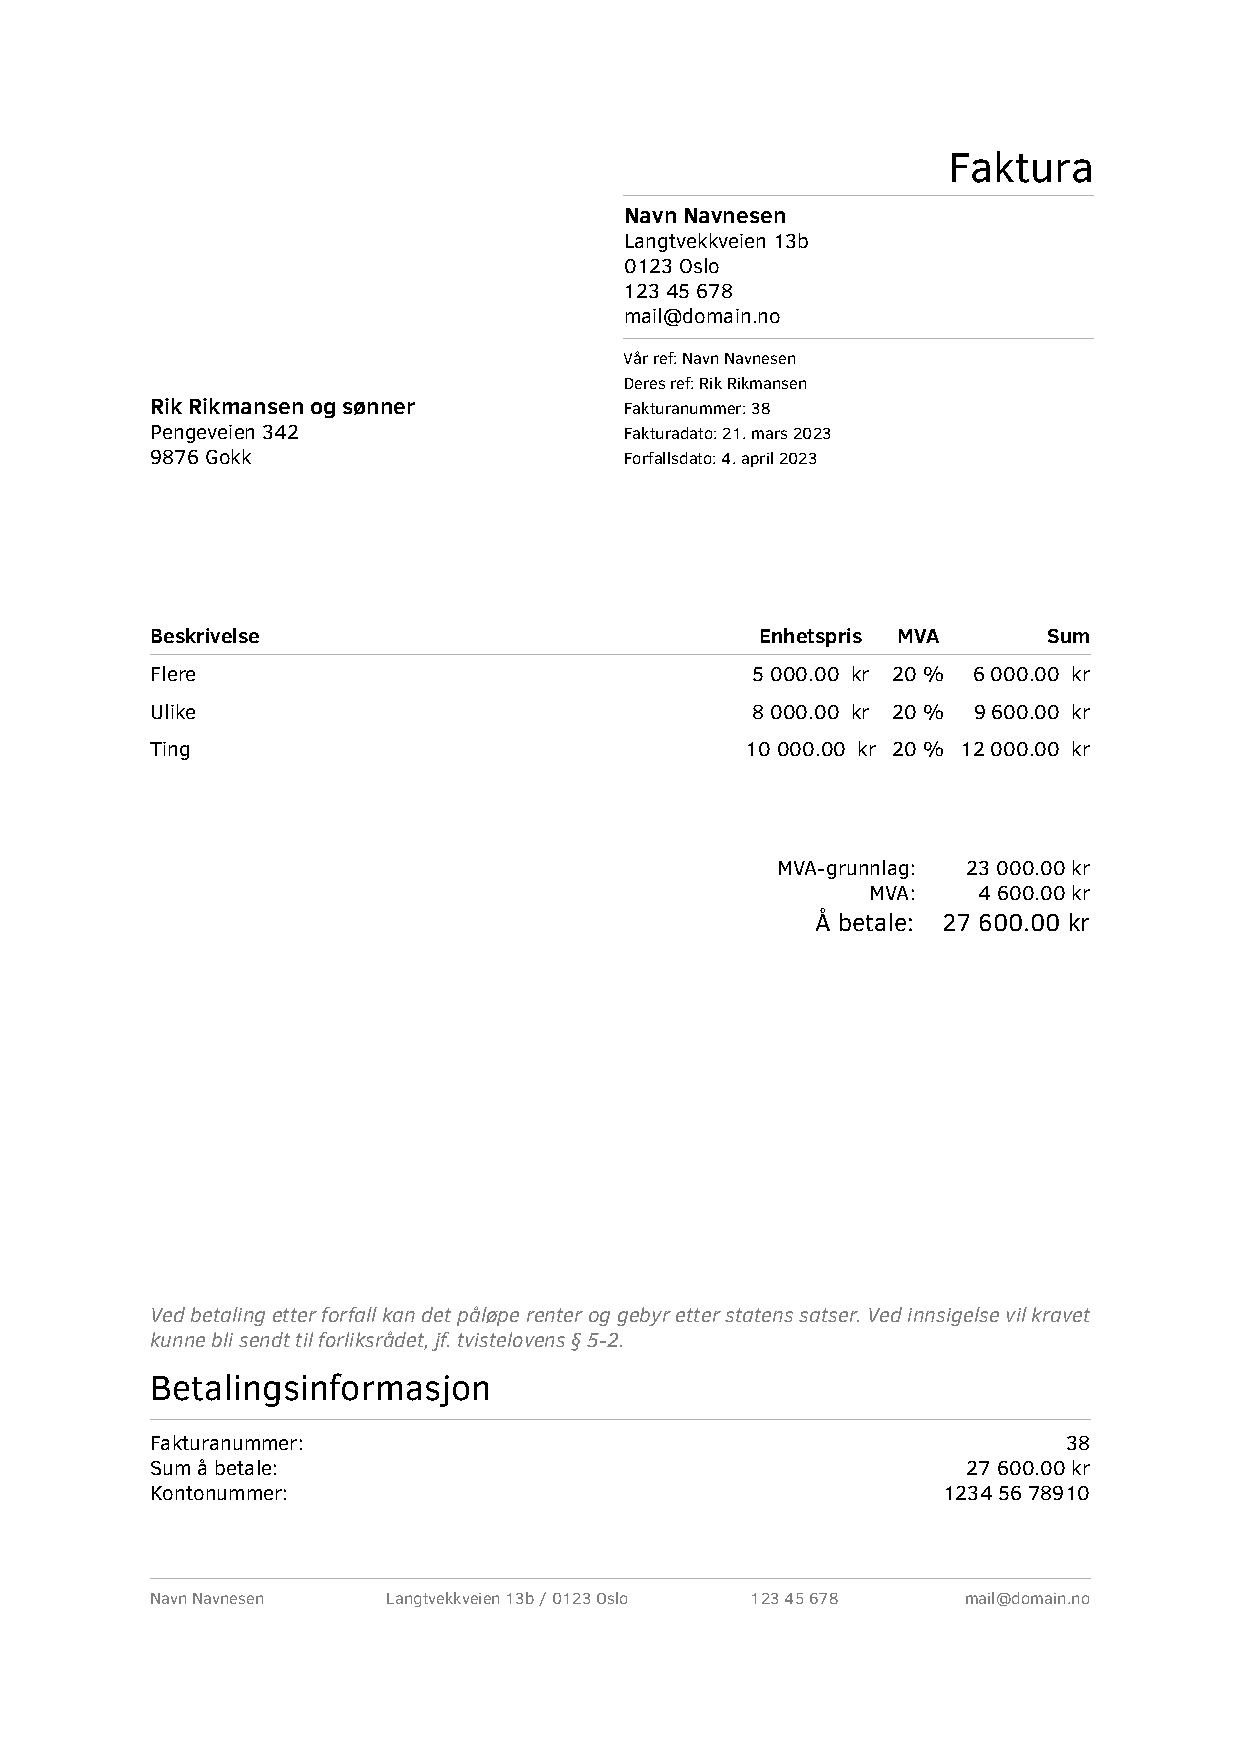
\includepdf{examples/norwegian.pdf}



\chapter{Licensing and legal stuff}
The package is licensed under the GPL v3 license. The full license is found on the GitHub page of the project, but the short version is that you may use this package freely, and without any charge. Even for commercial purposes. The only thing I ask in return is that if you improve the source code for the package in any way, I want you to send me those changes back. Either in an email, or as a pull request on GitHub. That way I can consider if I want to add your changes to the official package.



\end{document}
\grid
